\documentclass{article}
\usepackage[english]{babel}
\usepackage[a4paper,top=2cm,bottom=2cm,left=3cm,right=3cm,marginparwidth=1.75cm]{geometry}

\usepackage{amsmath}
\usepackage{graphicx}
\usepackage{subcaption}
\usepackage[colorlinks=true, allcolors=blue]{hyperref}

\title{DRMBM (1994) remake}
\author{Christopher Ashford}
\date{September 2022}

\begin{document}
\maketitle

\tableofcontents

\section{Analysis}

\subsection{Introduction and Background}

Dr Robotnik’s Mean Bean Machine is a 1994 Westernised port of Puyo Puyo for the Sega Genesis/Mega Drive. It is a game that I have enjoyed throughout my childhood on many different forms – cheap emulation consoles, the Sega Mega Drive Collection for Xbox 360, using Fusion emulator on PC among other forms. However, all of these present glaring issues that directly affect the enjoyment of the player – emulation consoles usually are slow with clunky controllers and are not good for much else and thus are not practical to use permanently; the Sega Mega Drive collection on Xbox 360 suffers with a noticeable input lag problem, with inputs sometimes taking hundreds of milliseconds to be processed, directly affecting how fast you can play; PC emulation either results in a small or blurry image and makes it difficult to play with others or share your scores and achievements.

The goal of this project is to solve these problems by creating a superior, native PC remake of the game. Everything in the original game shall work exactly as in the original, including re-constructing the algorithms used for the playstyles of the various AI opponents. I also intend to include many quality of life improvements to solve the problems listed about: multiple customisable input method and handling will be supported, many algorithmic optimisations shall be made to improve performance, graphics shall be upscaled in a way that remains a crisp pixel look instead of introducing blur, an SQL web server will allow score and time leaderboards to exist and a replay file system shall be introduced to allow players to easily share gameplay. This project exists to create a superior version of DRMBM for a new generation to enjoy, as well as offering a way for modern Puyo Puyo players to enjoy the OPP rule set on modern devices.

If the goals above are reached, further extension goals include the introduction of my own custom AI opponents with algorithms designed for optimal, “perfect” gameplay and the use of web sockets to facilitate real-time online matches between two remote players.

\subsection{Alternative Solutions}

In this section I shall present my research on other Puyo Puyo games, compare the advantages and disadvantages of different versions from the perspective of the end user and take inspiration for my own project.

\subsubsection{Emulation}

\begin{figure}[h]
\centering
\begin{subfigure}{0.49\textwidth}
\centering
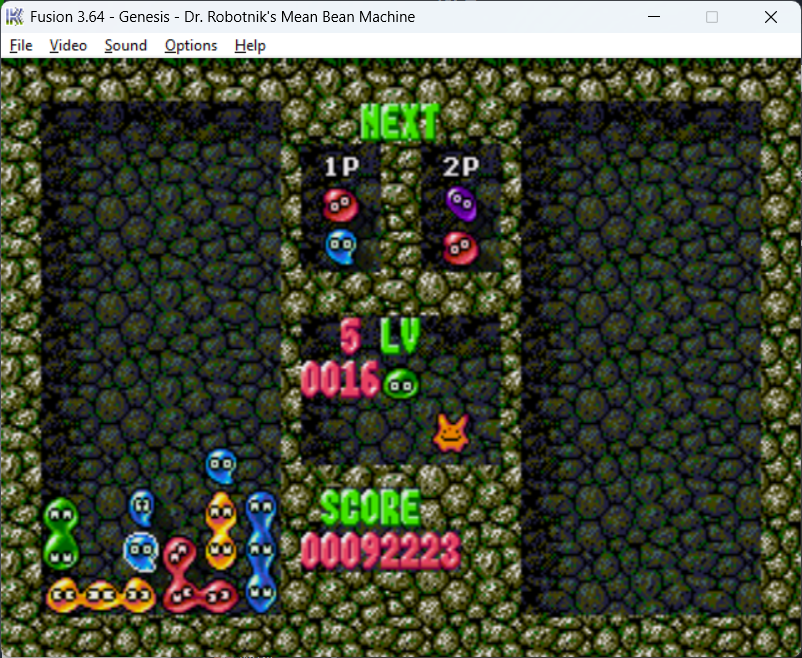
\includegraphics[width = \textwidth]{emulator1.png}
\caption{Fusion emulator}
\label{fig:emu1}
\end{subfigure}
\begin{subfigure}{0.45\textwidth}
\centering
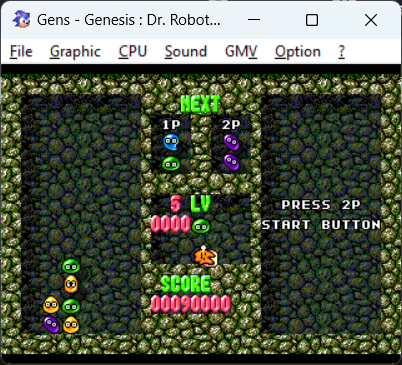
\includegraphics[width = \textwidth]{emulator2.png}
\caption{Gens emulator}
\label{fig:emu2}
\end{subfigure}
\caption{Some examples of emulators running the game}
\label{fig:combined}
\end{figure}

Link: cannot be provided due to specialised hardware being required to dump the ROM. Yet another disadvantage.

Many different emulators exist for the Sega Mega Drive, such as Fusion or Gens shown above, or the official Sega emulator that can be found on Steam. These are programs that accept a binary ROM dump of the original cartridge and attempt to emulate the code.
\vspace{0.3cm}

Advantages:

\begin{itemize}
    \renewcommand\labelitemi{--}
    \item Convenient for mass production and distribution.
    Sega can create one Mega Drive emulator and release an entire of library of games that use the same program
    \item True to the original experience.
    Since you are playing a copy of the original game, you can be sure you are getting an authentic experience
    \item While clunky, save states allow you to save high scores and progress through the story, as well as letting you manipulate sequences of beans
\end{itemize}

Disadvantages: 

\begin{itemize}
    \renewcommand\labelitemi{--}
    \item Resolution is locked at the console’s original and upscaling is blurry and unappealing
    \item Very static and not customisable. It is incredibly difficult to edit a ROM if you wanted to play with, for example, different handling or textures
    \item Saving progress is difficult
    \item Emulators are difficult to run and can easily lag on lighter hardware, running the game at higher levels can struggle on older processors
    \item It is impossible to play with friends remotely (or if it is possible, then it’s too difficult for the average user to achieve)
\end{itemize}

\subsubsection{B Puyo}

\begin{figure}[h]
\centering
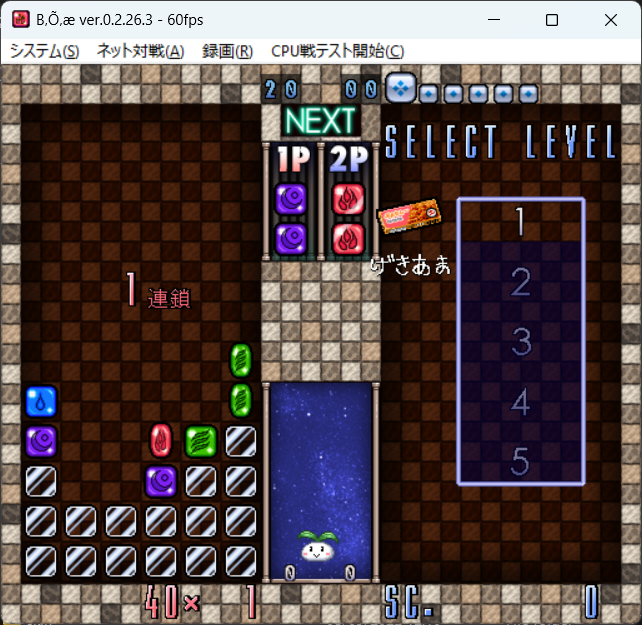
\includegraphics[width=0.3\textwidth]{bpuyo.png}
\caption{\label{fig:bpuyo}A screenshot of B Puyo. Some text is broken running on an English computer.}
\end{figure}
\begin{figure}[h]
\centering
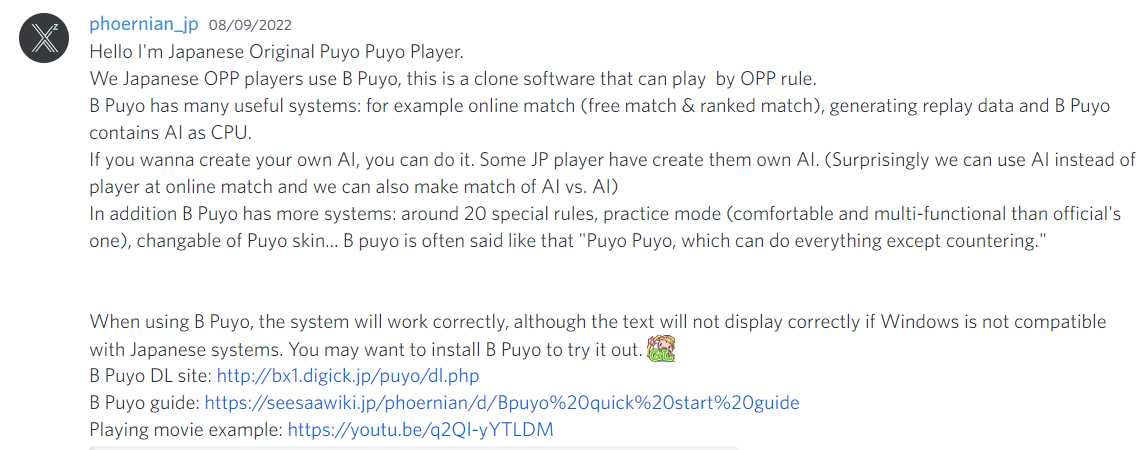
\includegraphics[width=1\textwidth]{discord.png}
\caption{\label{fig:discord}Information about B Puyo from a well known Japanese player.}
\end{figure}
Link: \href{http://bx1.digick.jp/puyo/dl.php}{http://bx1.digick.jp/puyo/dl.php}

B puyo is a popular online Puyo-clone recommended to me by the Japanese community.
\vspace{0.3cm}

Advantages:

\begin{itemize}
    \renewcommand\labelitemi{--}
    \item Custom textures, custom AI, custom rules, custom anything really
    \item Easy to use online multiplayer
    \item Great performance as a native PC program

\end{itemize}

\vspace{3cm}

Disadvantages: 

\begin{itemize}
    \renewcommand\labelitemi{--}
    \item Will only run on Windows, excluding Mac and Linux users
    \item The entire thing is in Japanese, with no translation options. Furthermore, servers are in Japan, creating ping issues for non-Japanese players. This is great for the Japanese community, but unfortunately disadvantages me as a Western player
    \item The resolution is locked to being a small window, making it uncomfortable to use on high-resolution displays
\end{itemize}

\subsubsection{Project GelaVolt}

\begin{figure}[h]
\centering
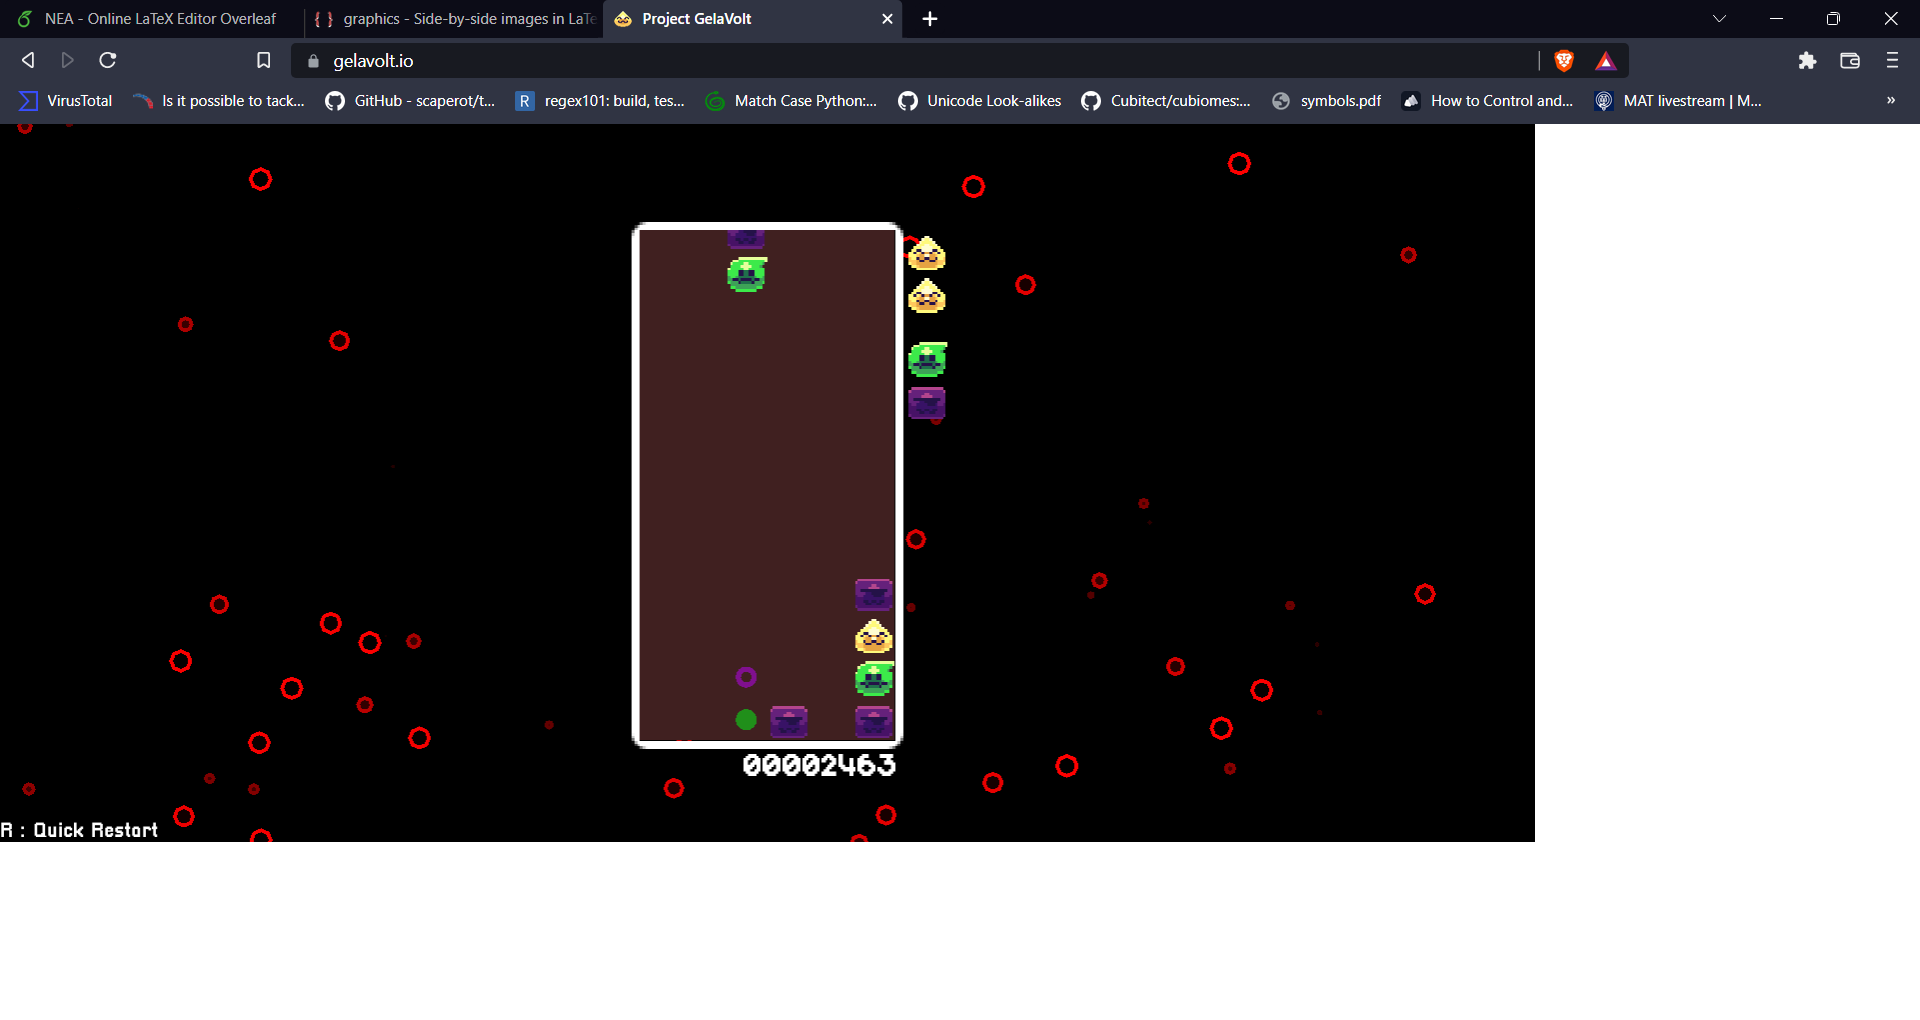
\includegraphics[width=1\textwidth]{gelavolt.png}
\caption{\label{fig:gelavolt}A screenshot of GelaVolt running in a chromium-based web browser.}
\end{figure}
Link: \href{https://gelavolt.io/}{https://gelavolt.io/}

To quote the game’s creator, “Project GelaVolt is a modern, techno-themed pixel art fangame of SEGA's Puyo Puyo series, one of Japan's most successful puzzle fighter franchises. Currently, GelaVolt is focused on the competitive aspects of the game and it's intended purpose is to help introduce people and help people get better at Puyo Puyo. However, if all goes well, GelaVolt will become a free alternative that plans to solve some of the communities problems: lack of players, lack of crossplay and lack of general quality netcode.” It is a Puyo-clone written in Haxe that runs in browsers.
\vspace{0.3cm}

Advantages:

\begin{itemize}
    \renewcommand\labelitemi{--}
    \item Appealing design
    \item Is lightweight and capable of running well in browsers
    \item Supports many different control schemes out of the box (controller, keyboard, etc.)
    \item Only version I’ve played that has hard drop
\end{itemize}

\vspace{0.7cm}

Disadvantages: 

\begin{itemize}
    \renewcommand\labelitemi{--}
    \item Multiplayer is in the works but is currently not supported at the time of writing
    \item Things such as textures are not customisable
    \item Is unstable and crashes regularly
\end{itemize}

\subsubsection{Puyo Puyo Tetris 2}

\begin{figure}[h]
\centering
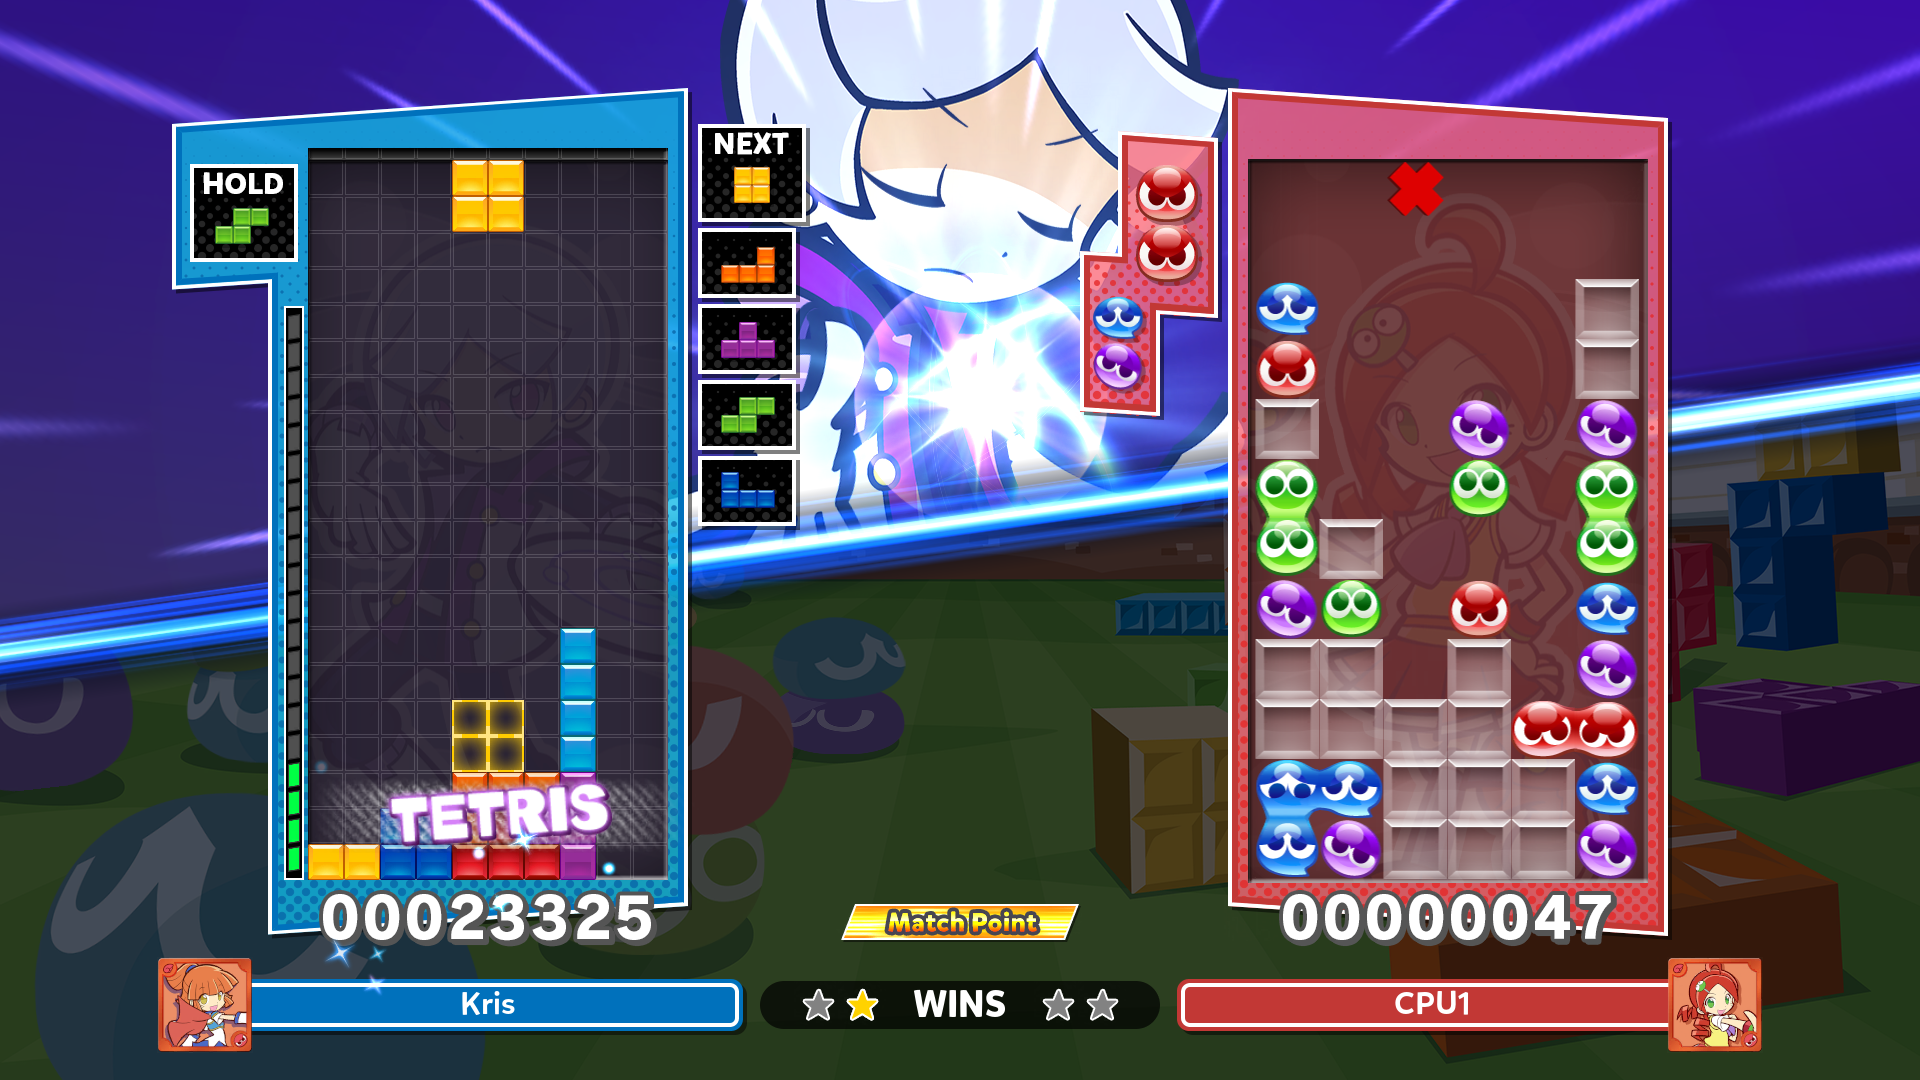
\includegraphics[width=1\textwidth]{ppt2.png}
\caption{\label{fig:ppt2}A screenshot of a versus battle, I'm playing Tetris and the CPU is playing Puyo Puyo.}
\end{figure}
Link: \href{https://store.steampowered.com/app/1259790/Puyo_Puyo_Tetris_2/}{https://store.steampowered.com/app/1259790/Puyo\_Puyo\_Tetris\_2/}

Puyo Puyo Tetris 2 is the latest Puyo Puyo game released by Sega and combines Puyo Puyo gameplay with Tetris, allowing players of both games to seamlessly play against one another. It has a full story and online mode.
\vspace{1cm}

Advantages:

\begin{itemize}
    \renewcommand\labelitemi{--}
    \item Cutesy art style is appealing to many, but can be swapped out with unlockable designs
    \item Being an official release, it is very stable with a consistent online multiplayer
    \item CPU opponents
    \item Fully voice-acted story with unique and creative characters
    \item Active modding community
\end{itemize}

Disadvantages: 

\begin{itemize}
    \renewcommand\labelitemi{--}
    \item Ranked multiplayer is fundamentally flawed as leaving matches is not punished
    \item CPU opponents fail to provide a challenge
    \item The game is very expensive, whereas all other options listed above are free
    \item Tsu ruleset, unable to be changed
\end{itemize}

\subsection{Input, Data Processing, Output}

\begin{figure}[h]
\centering
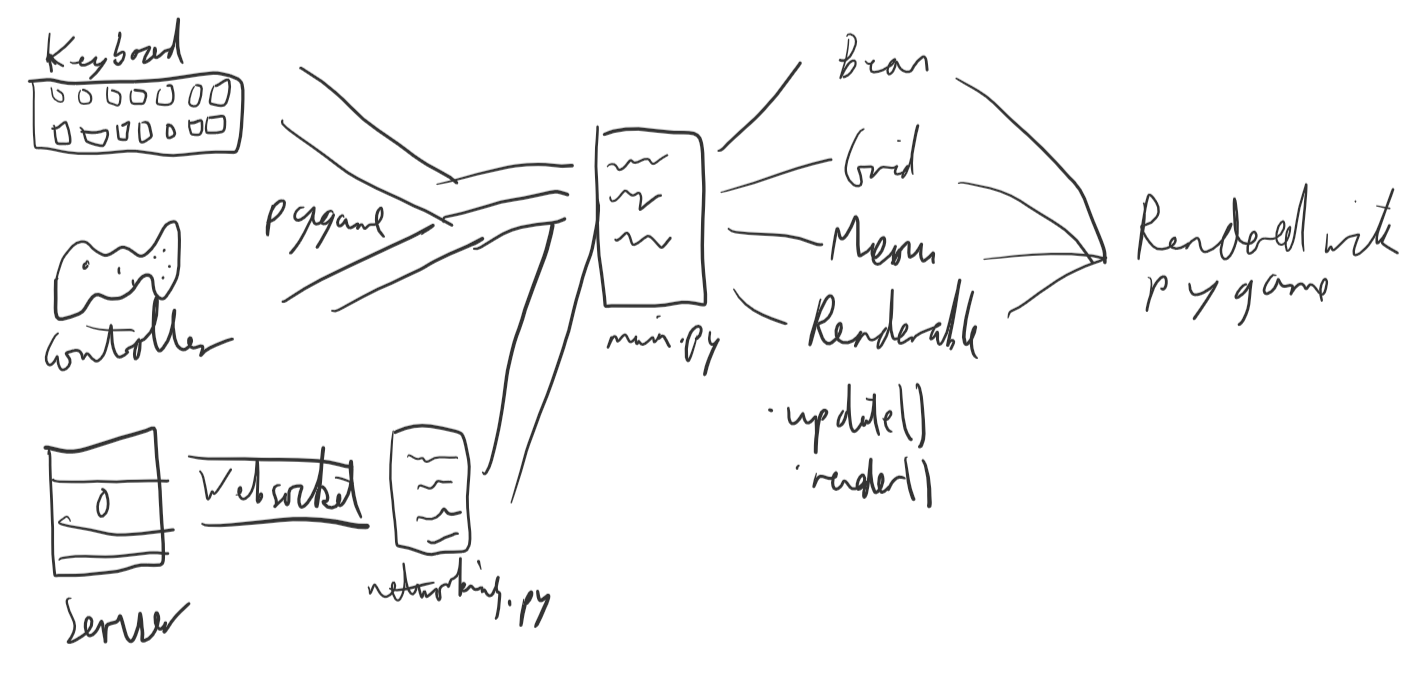
\includegraphics[width=1\textwidth]{idpo.png}
\caption{\label{fig:idpo}A simple diagram demonstrating the input the program will take from various input devices such as keyboards and controllers, in addition to data received from web a real-time websocket where applicable. This is then processed by a main script which makes the data available to various renderable classes, updates and renders them before pygame is used to display the output on the screen. This is heavily simplified.}
\end{figure}

\subsection{Goals}

The easiest way to demonstrate the various goal and features is to demonstrate what I intend to plan to add in each version. These versions will not necessarily be completed within the project's time-span as they may be extension goals and will be specified as such.

Version 0.1 alpha

The base version of the project. Should implement basic gameplay and functionality.
\begin{itemize}
    \renewcommand\labelitemi{--}
    \item Introduce basic start up script. Introduce basic repair and update functionality by hashing files and comparing against a simple HTTPS GET API.
    \item Establish a basis for which to build the program up on. Initialise screen class that is rendered with while true loop and dynamically creates renderable objects with both update and render class methods. These are called in that order every frame. Update passes in input data, which the screen class is responsible for retrieving at the start of the frame.
    \item Create classes and methods required for basic gameplay. The easiest thing to create will be "exercise mode", a simple single-player "play forever" scoring mode. Things such as leaderboards will not be introduced yet, only the basic gameplay.
    \item Code all the algorithms required for basic gameplay, such as randomly generating bean pairs and identifying colour groups without excessive iteration. Establish important gameplay constants such as the formula for fall speed, scoring, garbage puyos and important handling settings such as DAS and ARR.
\end{itemize}

Version 0.2 alpha

Introduce the necessary code for multiplayer (handles code for games against an opponent i.e. CPU, NOT CODE FOR ONLINE MULTIPLAYER.) and code all AI opponents into the game.
\begin{itemize}
    \renewcommand\labelitemi{--}
    \item Code algorithms for all 13 AI opponents included in the story mode. This should be done in a modular fashion, such that it is easy for I, or someone attempting to modify the game, to create a new opponent with unique AI.
    \item Introduce code to accept different input methods.
    \item With this multiplayer code in place, it should not be difficult to add local 2 player mode. This will then mean the game has all modes from the original.
    \item Iron out niche mechanics such as Has Bean and Big Bean.
    \item Introduce a simple REST API based SQL score and time leaderboard for exercise mode
\end{itemize}

Version 0.3 beta

Introduce non-essential cosmetic features that will make the program useable and user friendly such as menus and transition animations. This version will be the first that will be released to a select few individuals for testing and ironing out of bugs. This version will meet all of the base requirements for the project, further updates shall exist as extension goals.
\begin{itemize}
    \renewcommand\labelitemi{--}
    \item Add menus and settings
    \item Fully animate sprites and transitions, allow the whole game to be accessible without the use of debug commands
    \item Create a simple C++ installation script that installs the game and it's pre-requisites for easy distribution and testing
\end{itemize}

Version 0.4 beta

This version will focus on the introduction of online multiplayer through web sockets and server programming. Being an extension goal, the method behind achieving this is more vague and shall be revealed if we get to that point.

\vspace{0.3cm}

Version 0.5 beta

If I have time I will attempt to create an ideal algorithm for playing the game itself, a perfect opponent to train against, and make this available to players. Bug fixes and finalisations in addition to taking requests from players about potentially adding more gamemodes. Bar the algorithm creation this is probably beyond the scope of this project.
\end{document}

% NOTES
% SECTION - \section
% SUBSECTION - \subsection
% IMAGE
%\begin{figure}
%\centering
%\includegraphics[width=0.3\textwidth]{frog.jpg}
%\caption{\label{fig:frog}This frog was uploaded via the file-tree menu.}
%\end{figure}
% LINK - \href
% REFERENCES - \bibliographystyle{alpha}
% \bibliography{sample} WHERE SAMPLE IS A FILE sample.bib THAT LOOKS LIKE THIS
%@article{greenwade93,
%    author  = "George D. Greenwade",
%    title   = "The {C}omprehensive {T}ex {A}rchive {N}etwork ({CTAN})",
%    year    = "1993",
%    journal = "TUGBoat",
%    volume  = "14",
%    number  = "3",
%    pages   = "342--351"
%}
% CITE WITH \cite{greenwade93}
% EXAMPLE TABLE
%\centering
%\begin{tabular}{l|r}
%Item & Quantity \\\hline
%Widgets & 42 \\
%Gadgets & 13
%\end{tabular}
% LIST
%\begin{itemize}
%\item Like this,
%\item and like this.
%\end{itemize}
% itemize FOR BULLET POINTS enumerate FOR NUMBERS